\documentclass[12pt]{article} 
\usepackage{fullpage} 
\usepackage[affil-it]{authblk} 
\newcommand{\tab}{\hspace*{2em}}
\usepackage{graphicx} 
\usepackage{caption}
\usepackage{subcaption}
\graphicspath{ {.} } 
\usepackage{float} 
\usepackage{url} 
\usepackage{mhchem}
\usepackage{siunitx}

\begin{document} 

\title{Comparing CENNS detector simulations of Geant4 and MCNP} 

\author[1]{Jan P. Adam} 
\author[2]{Kate Scholberg} 
\affil[1]{Technische Universit\"at Dortmund, Fakult\"at Physik, Dortmund, Germany} 
\affil[2]{Duke University, Department of Physics, Durham, NC 27705} 
\date{October 4, 2014} 

\maketitle
\begin{abstract}
The Spallation Neutron Source (SNS) at Oak Ridge National Laboratory is also a neutrino source. The Duke Neutrino Group build a detector prototype to observe coherent elastic neutrino-nucleus scattering (CENNS), a process that has been predicted but never observed so far. Beforehand the detector was simulated with the MCNP-Polimi framework and the goal of this paper is to reproduce the results with Geant4.
\end{abstract}
\newpage

\section{Introduction}



\section{Simulation set up}

The Geant4 simulation toolkit was used to reproduce the results of. The detector set up can be seen in figure \ref{}. The detector's core consists of a lead cube (\SI{50}{cm} edge-length) with 4 holes that hold one EJ-301 scintillator, each. These are frustums of a cone and are made of pure liquid EJ-301 (\cf{C_8H_{10}}). The sides and the bottom of the lead cube are covered with a \SI{1}{cm} thick layer of EJ-200 a solid plastic scintillator (\cf{C_{10}H_{11}}]). Above the lead cube is a gap of \SI{21}{cm} followed by an Al-7075 plate with a thickness of \SI{2}{cm}. This plate shall reduce signals of cosmic neutrinos in the real detector. The whole setup is enclosed by a \SI{1}{m^3} water cube.

Neutrons are being generated randomly inside the lead with a random direction.

If a particle enters one of the scintillators and deposits energy, that amount will be converted into electron-equivalent energy by using the graph in figure \ref{fig:photonResponse}.

\begin{figure}[htbp]
	\centering
	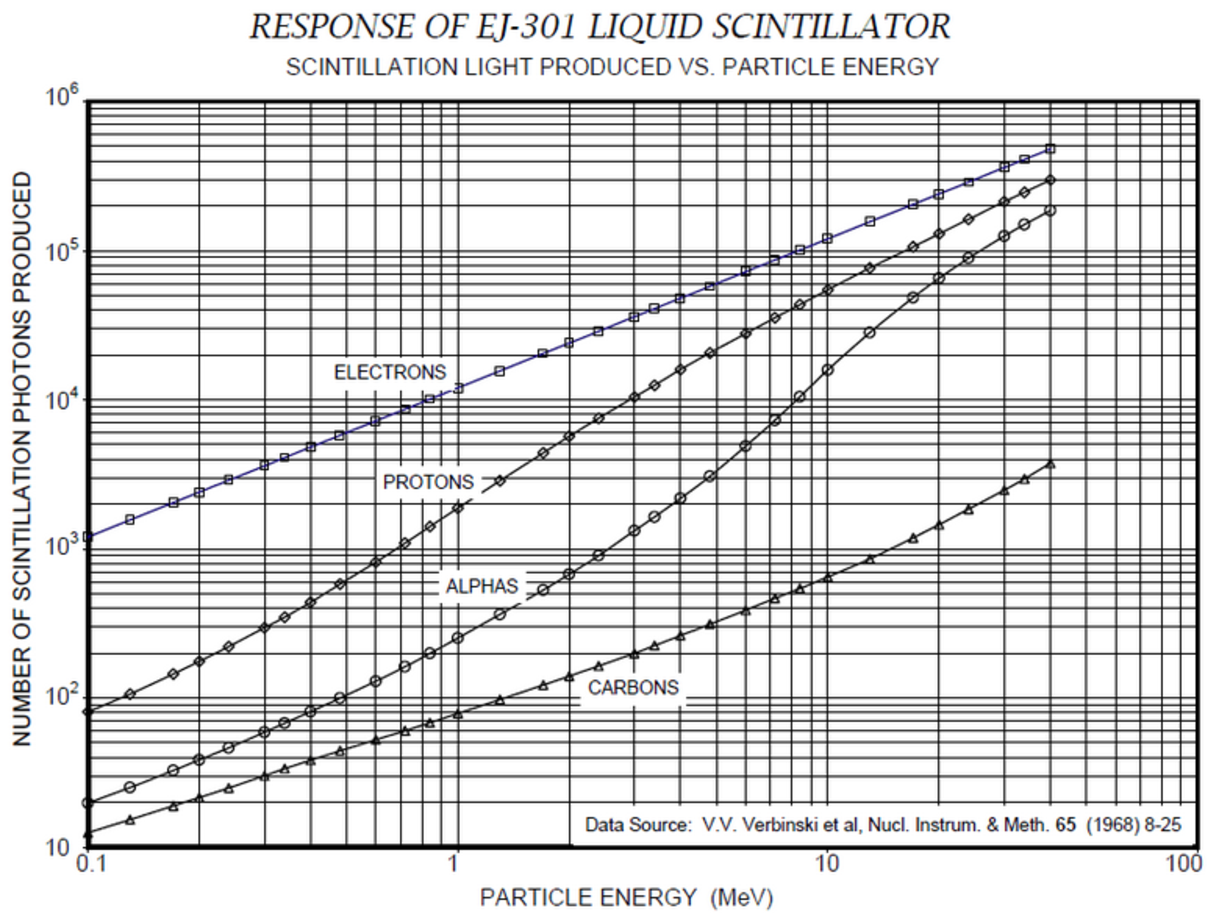
\includegraphics[width=0.7\textwidth]{./pics/scintillatorResponse.pdf}
	\caption{Photon response of the EJ-301 scintillator.}
	\label{fig:photonResponse}
\end{figure}
In addition to the four particles mentioned in this graph there is also a number of $\gamma$, $e^+$ and deuterons that enter the scintillator. Since $e^+$ have the same mass and charge as electrons and $\gamma$ will decay into $e^- + e^+$, both are treated as electrons. Deuterons will approximately emit a number of photons that lies in the middle between $p$ and $\alpha$. In approx. 0.5\% of the events the reaction 
\begin{align}
	\ce{n^1_0 + C^{12}_6 -> C^{13}_6 -> B^9_4 + \alpha^4_2 } 
\end{align}
can occur. Because this effect should be negligible, the electron-equivalent energy of the beryllium nucleus will not be calculated this case.

\section{Results and Discussion}

\subsection{Correct set up}

First of all, it was necessary to verify that the neutrons were generated in the correct volume. Figure \ref{} and \ref{} show that the particles were generated only inside the lead and not inside the holes which contain the scintillators. Figure \ref{} and \ref{} show that the direction of the neutrons is equally distributed.


\subsection{Efficiency}

An event will be marked as "valid" once the energy deposition in a single scintillator exceeds a given threshold in keVee.  Figure \ref{fig:efficiency30} and \ref{fig:efficiency100} show the percentage of events which were marked as "valid" at a given energy of the primary particle with an energy threshold of \SI{30}{keVee} and \SI{100}{keVee}.

 \begin{figure}[H]
 	\begin{subfigure}[t]{0.49\textwidth}
 		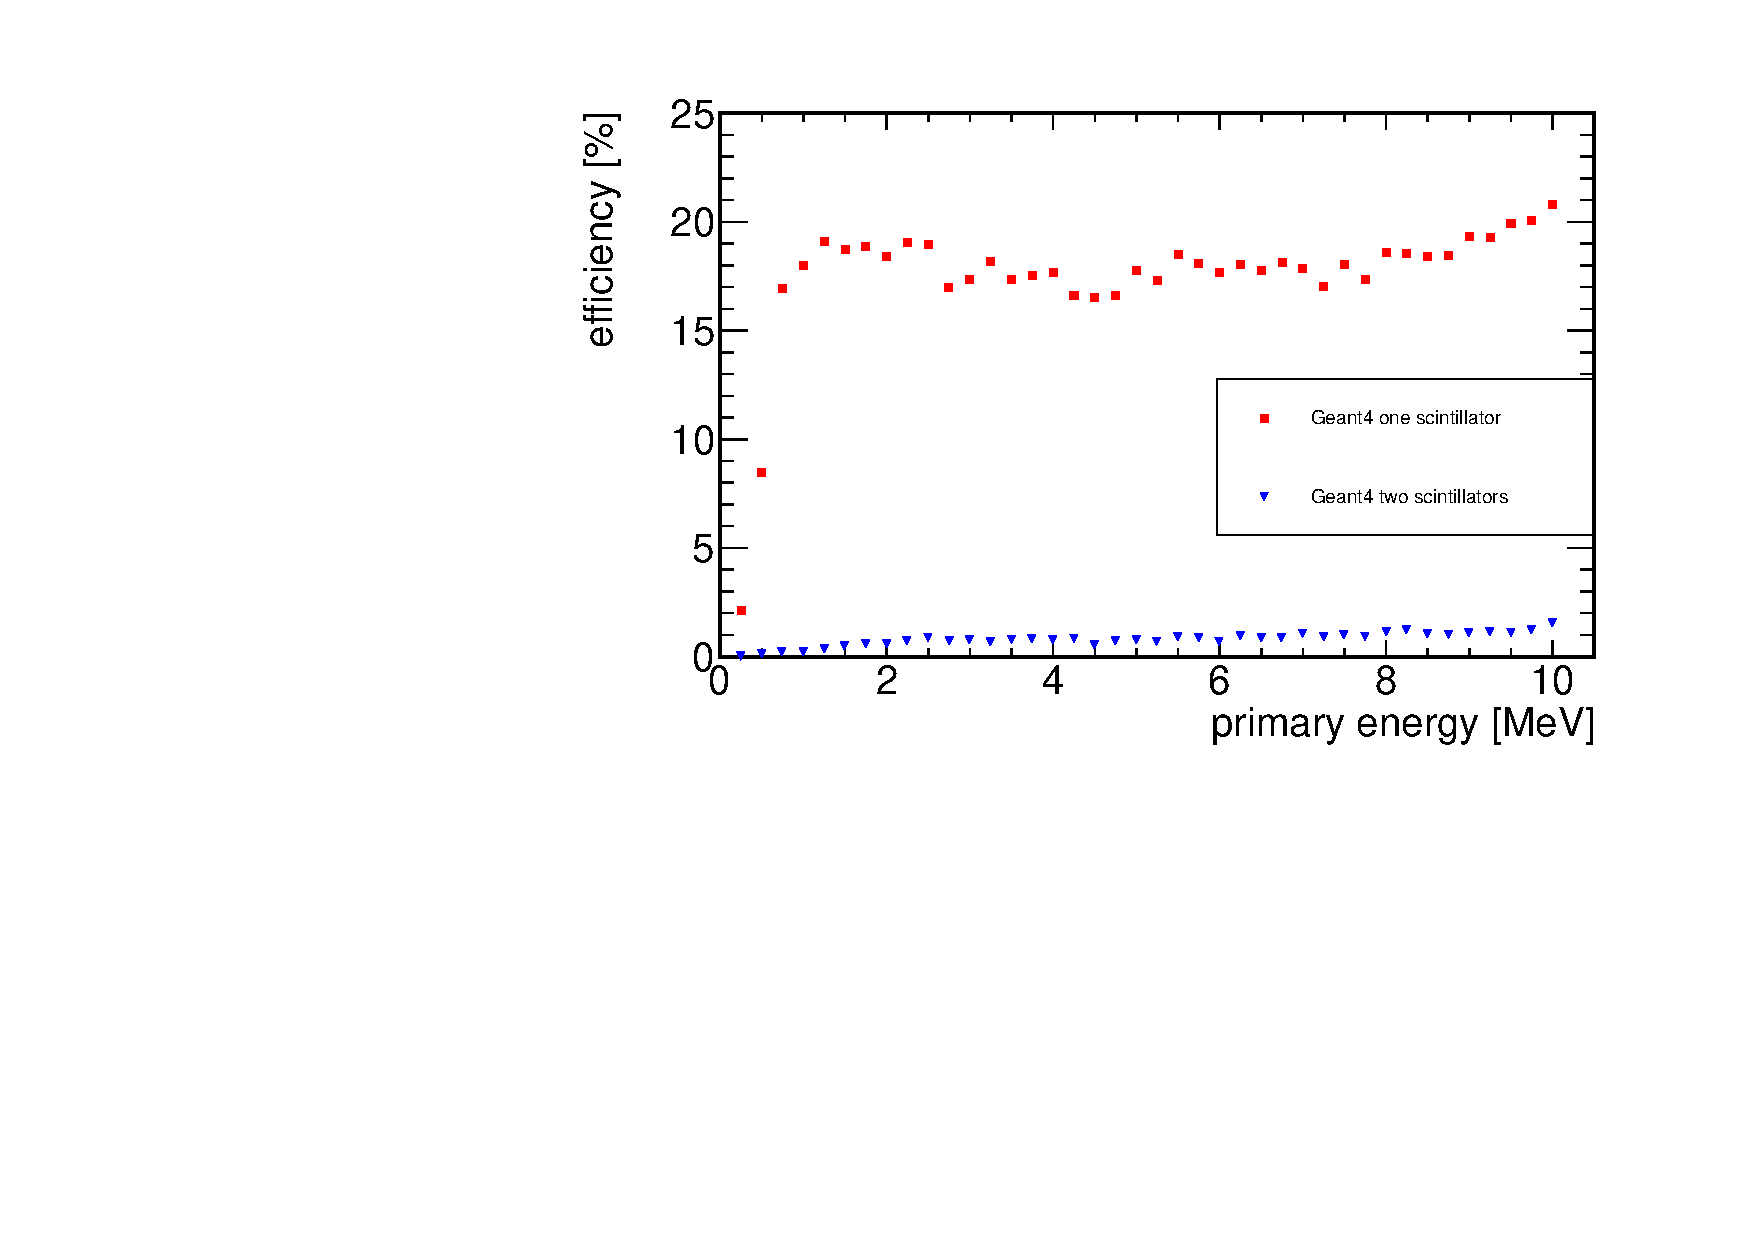
\includegraphics[trim = 0cm 0cm 0cm 1.15cm, clip,width=\textwidth]{pics/efficiencyGeant30.pdf}
 		\caption{Geant4 simulation.}
 	\end{subfigure}
 	\begin{subfigure}[t]{0.49\textwidth}
 		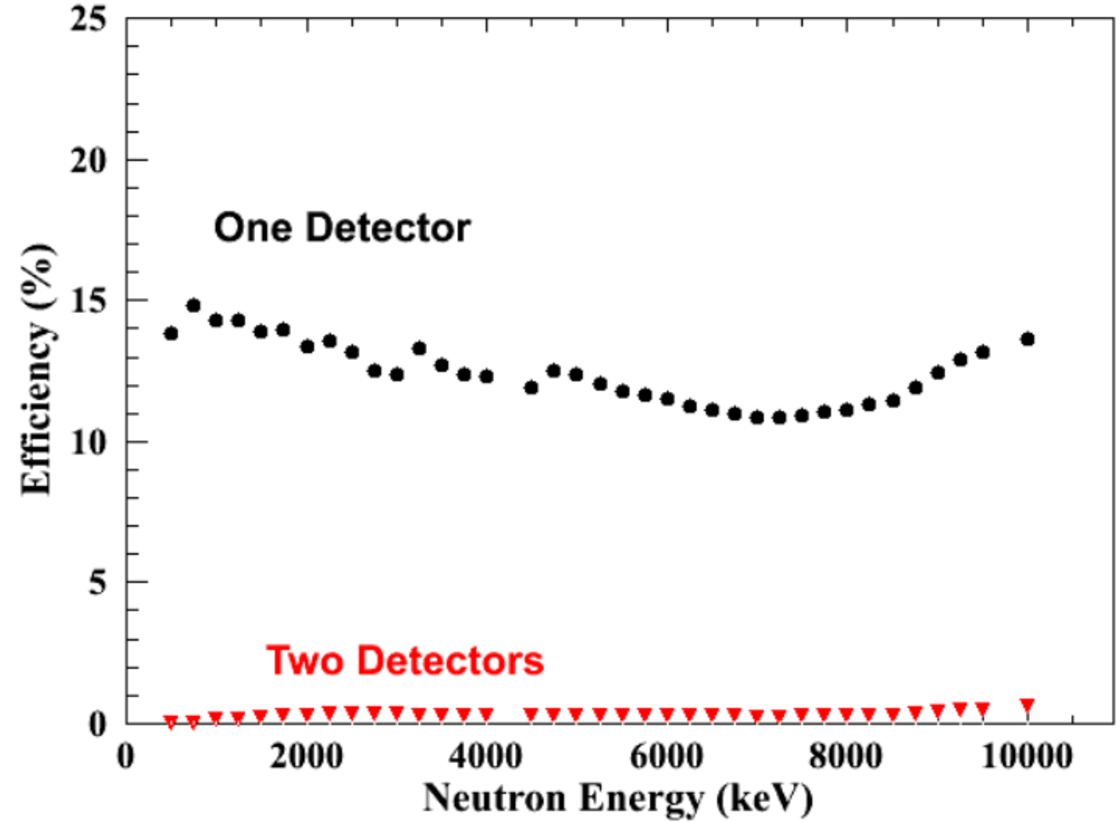
\includegraphics[trim = 0cm 0cm 0cm 1.15cm, clip, width=\textwidth]{pics/efficiency_MCNP30.pdf}
 		\caption{MCNP simulation.}
 	\end{subfigure}
 	\caption{Percentage of "valid" events for given monochromatic primary particles with a \SI{30}{keVee} threshold.}
 	\label{fig:efficiency30}
 \end{figure}
  \begin{figure}[H]
  	\begin{subfigure}[t]{0.49\textwidth}
  		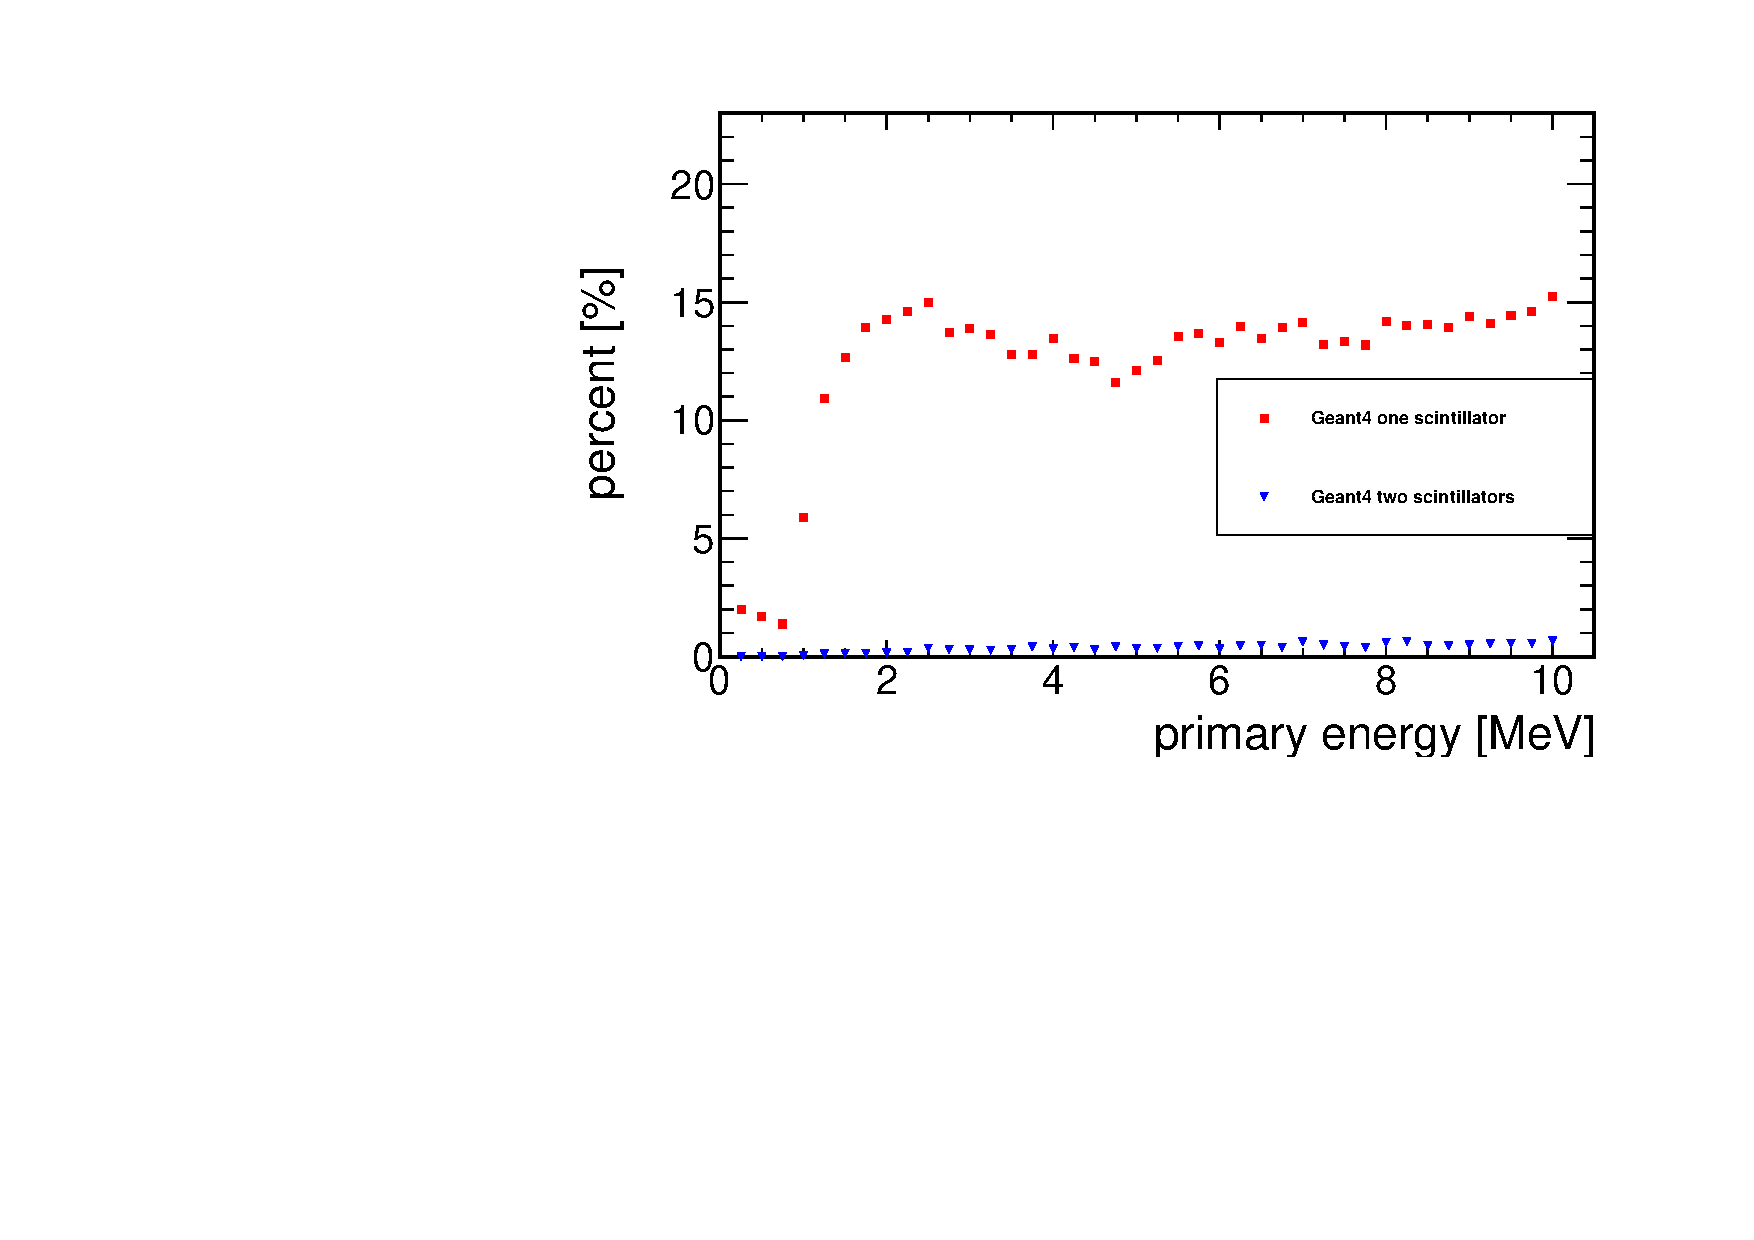
\includegraphics[trim = 0cm 0cm 0cm 1.15cm, clip,width=\textwidth]{pics/efficiencyGeant100.pdf}
  		\caption{Geant4 simulation.}
  	\end{subfigure}
  	\begin{subfigure}[t]{0.49\textwidth}
  		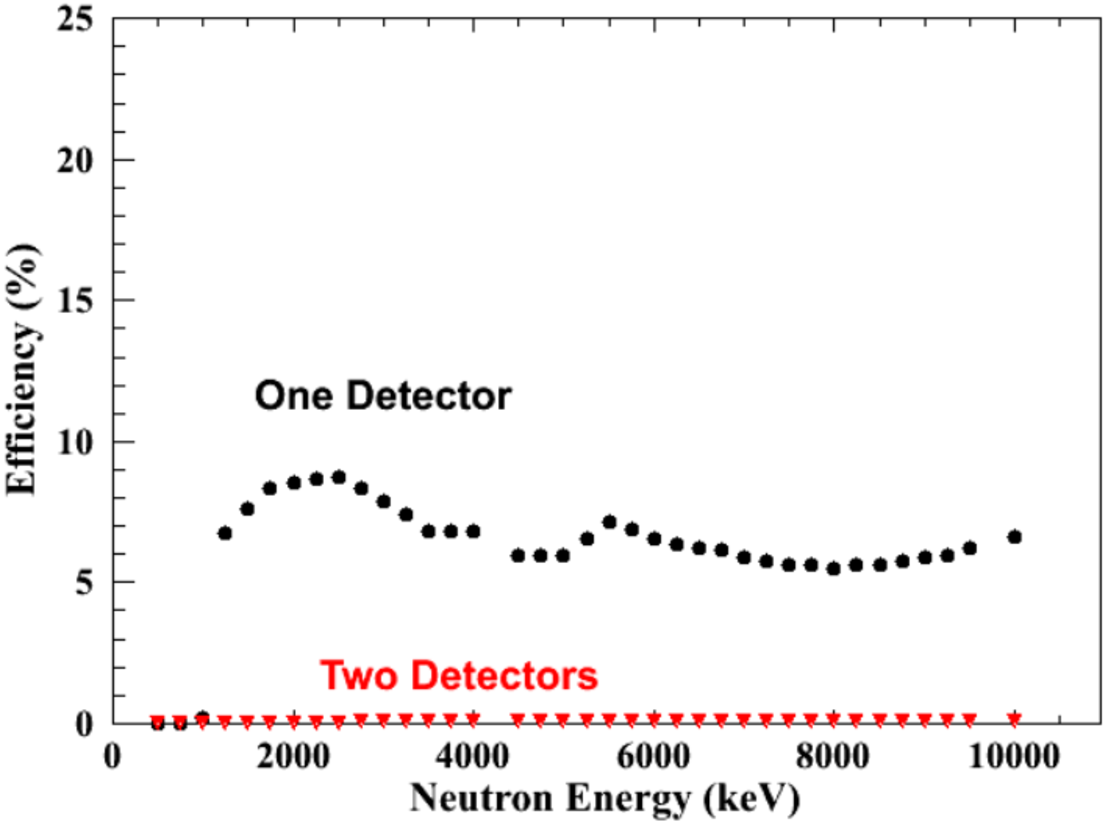
\includegraphics[trim = 0cm 0cm 0cm 1.15cm, clip, width=\textwidth]{pics/efficiency_MCNP100.pdf}
  		\caption{MCNP simulation}
  	\end{subfigure}
  	\caption{Percentage of "valid" events for given monochromatic primary particles with a \SI{100}{keVee} threshold.}
  	\label{fig:efficiency100}
  \end{figure}
  
 The efficiency of the Geant4 simulation is about 5\% higher. This might be a result of the superior tracking algorithms of Geant which will also track secondaries, whereas the MCNP simulation was run in neutron and photon mode only \ref{}. 
 
 Also, the scintillators were simulated as frustums of a cone instead as frustums of a hexagonal pyramid. This increases the cross-sectional area of each scintillator slightly and might result in more valid events.   
 
\subsection{Timing}

Figure \ref{fig:timing30} and \ref{fig:timing100} show a distribution of the arrival time of a signal. The neutron is being generated at $t=\SI{0}{ns}$ and a signal arrives once the energy deposition one scintillator exceeds a given threshold (\SI{30}{keVee} or \SI{100}{keVee}) for the first time.
 \begin{figure}[H]
 	\begin{subfigure}[t]{0.49\textwidth}
 	     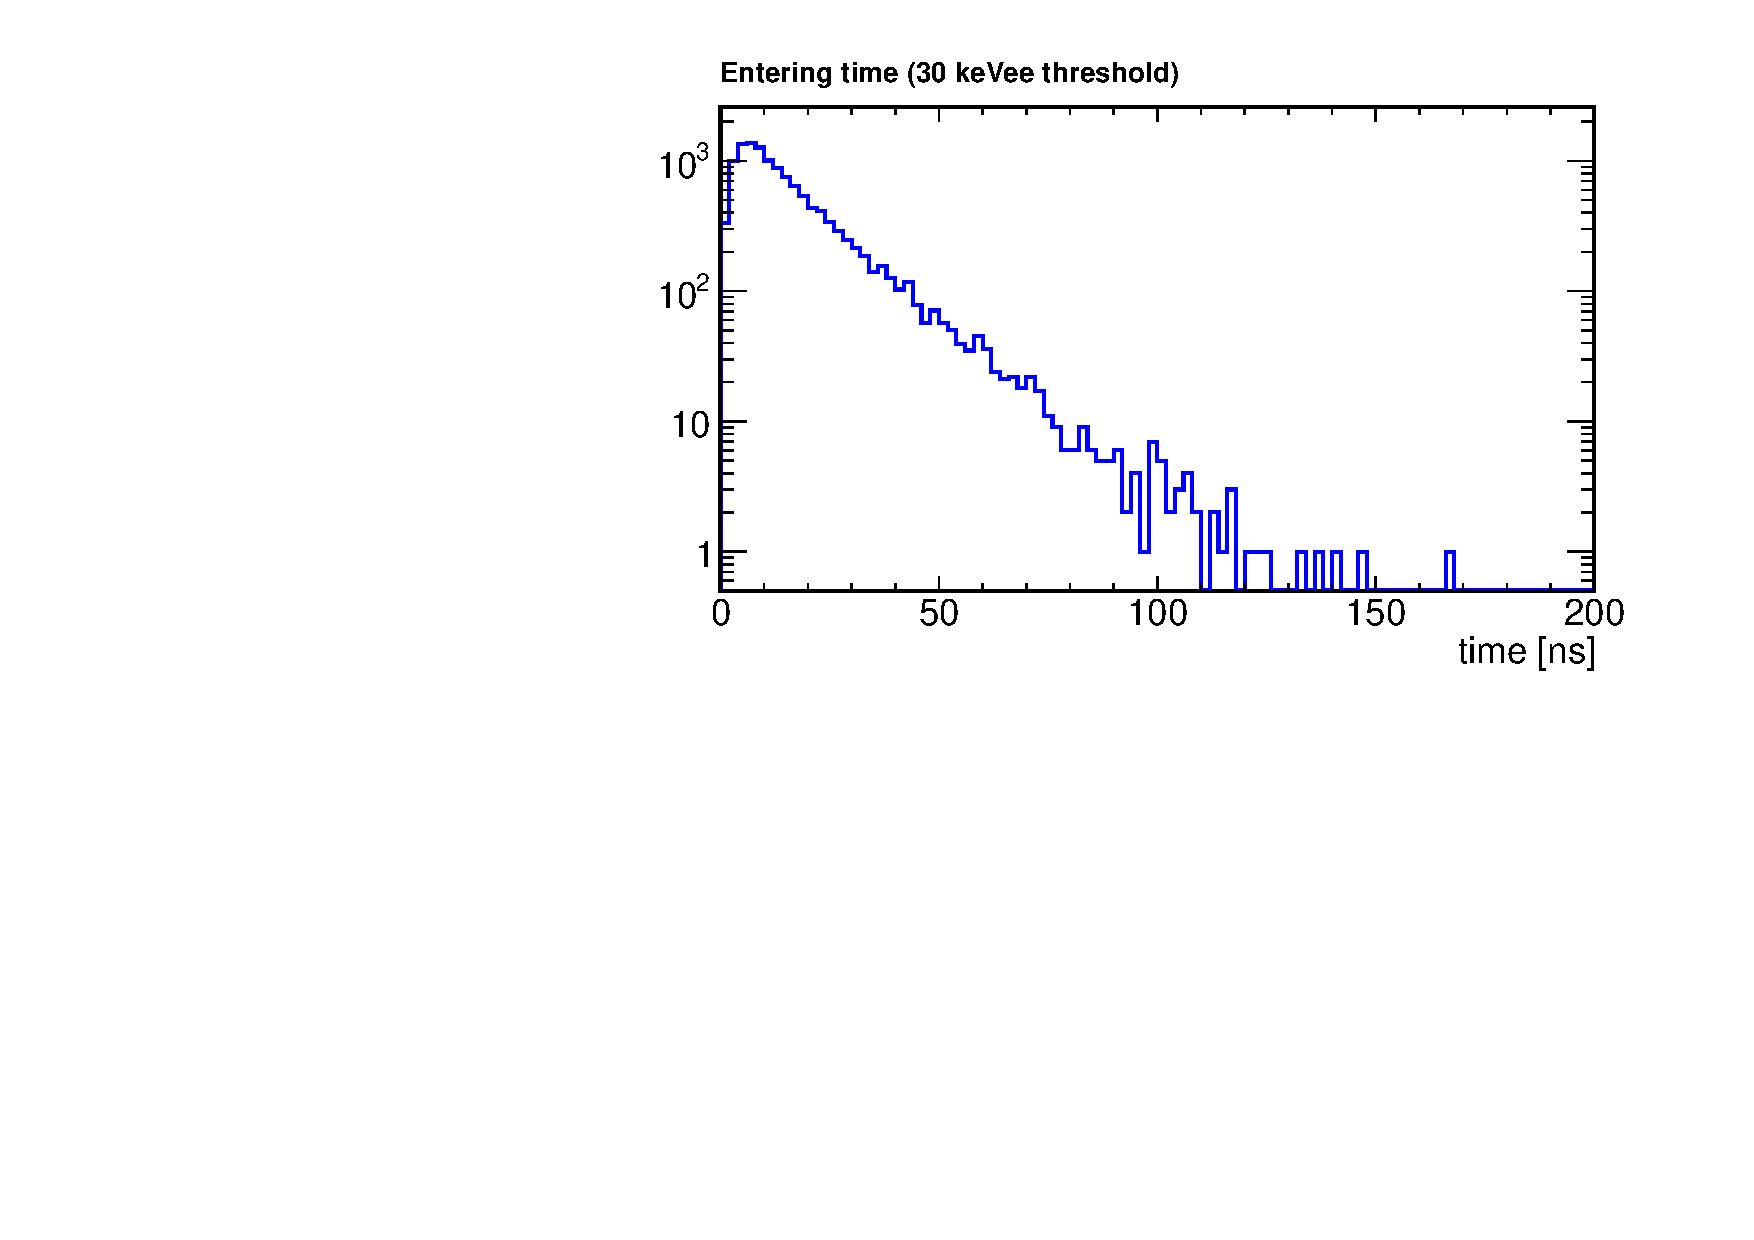
\includegraphics[trim = 0cm 0cm 0cm 1.15cm, clip, width=\textwidth]{pics/timing.pdf}
 		 \caption{Timing of Geant4 simulation.}
 	\end{subfigure}
 	\begin{subfigure}[t]{0.43\textwidth}
 	    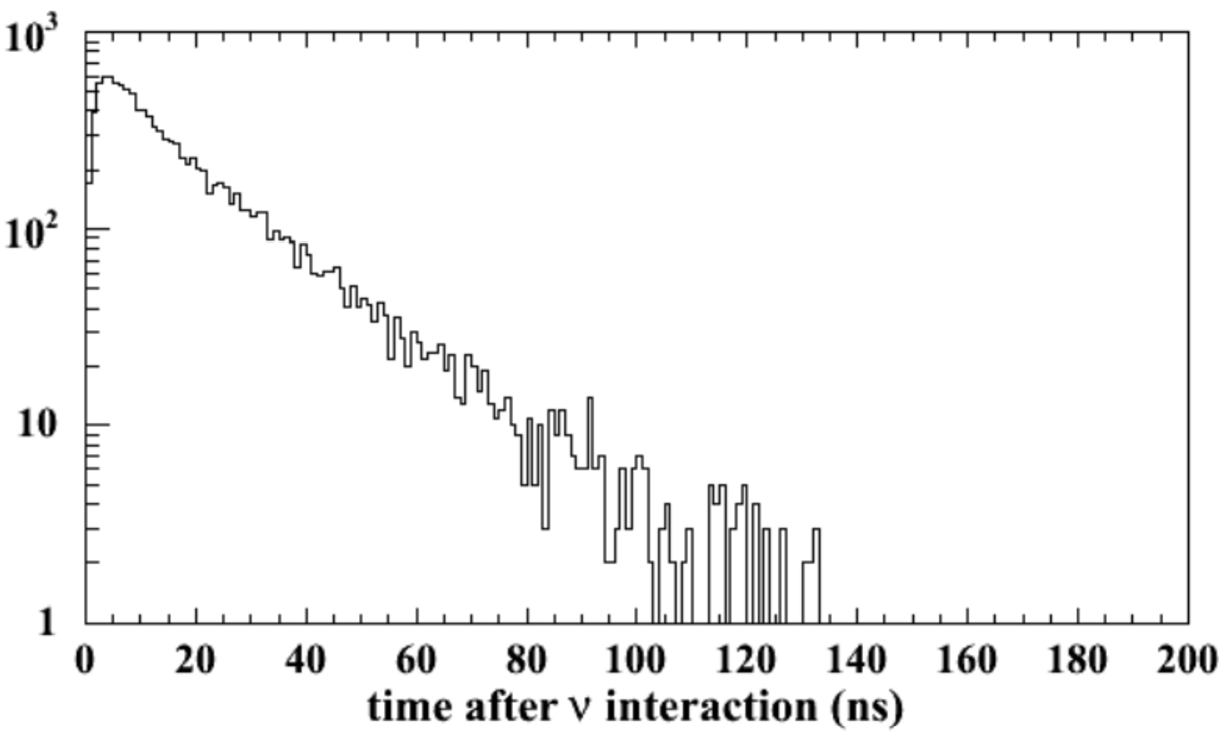
\includegraphics[width=\textwidth]{pics/timing_MCNP.pdf}
 		\caption{Timing of MCNP simulation.}
 	\end{subfigure}
 	\caption{Threshold \SI{30}{keVee}}
 	\label{fig:timing30}
 \end{figure}

The timing graphs of both, Geant4 and MCNP simulation, show a dropoff at \SI{0}{ns} due to the threshold and end somewhere between \SI{100}{ns} and \SI{140}{ns}.  

\subsection{Energy deposition}

Finally, the energy deposition of both simulations are being compared. Figure \ref{fig:photonResponse} provided the necessary data to convert the energy to keV electron equivalent (keVee). As mentioned before, $\gamma$ and $e^+$ are treated as $e^-$ and deuterons lie in the middle between $p$ and $\alpha$. Seldom particles like beryllium will be ignored.

 \begin{figure}[H]
 	\begin{subfigure}[t]{0.49\textwidth}
 		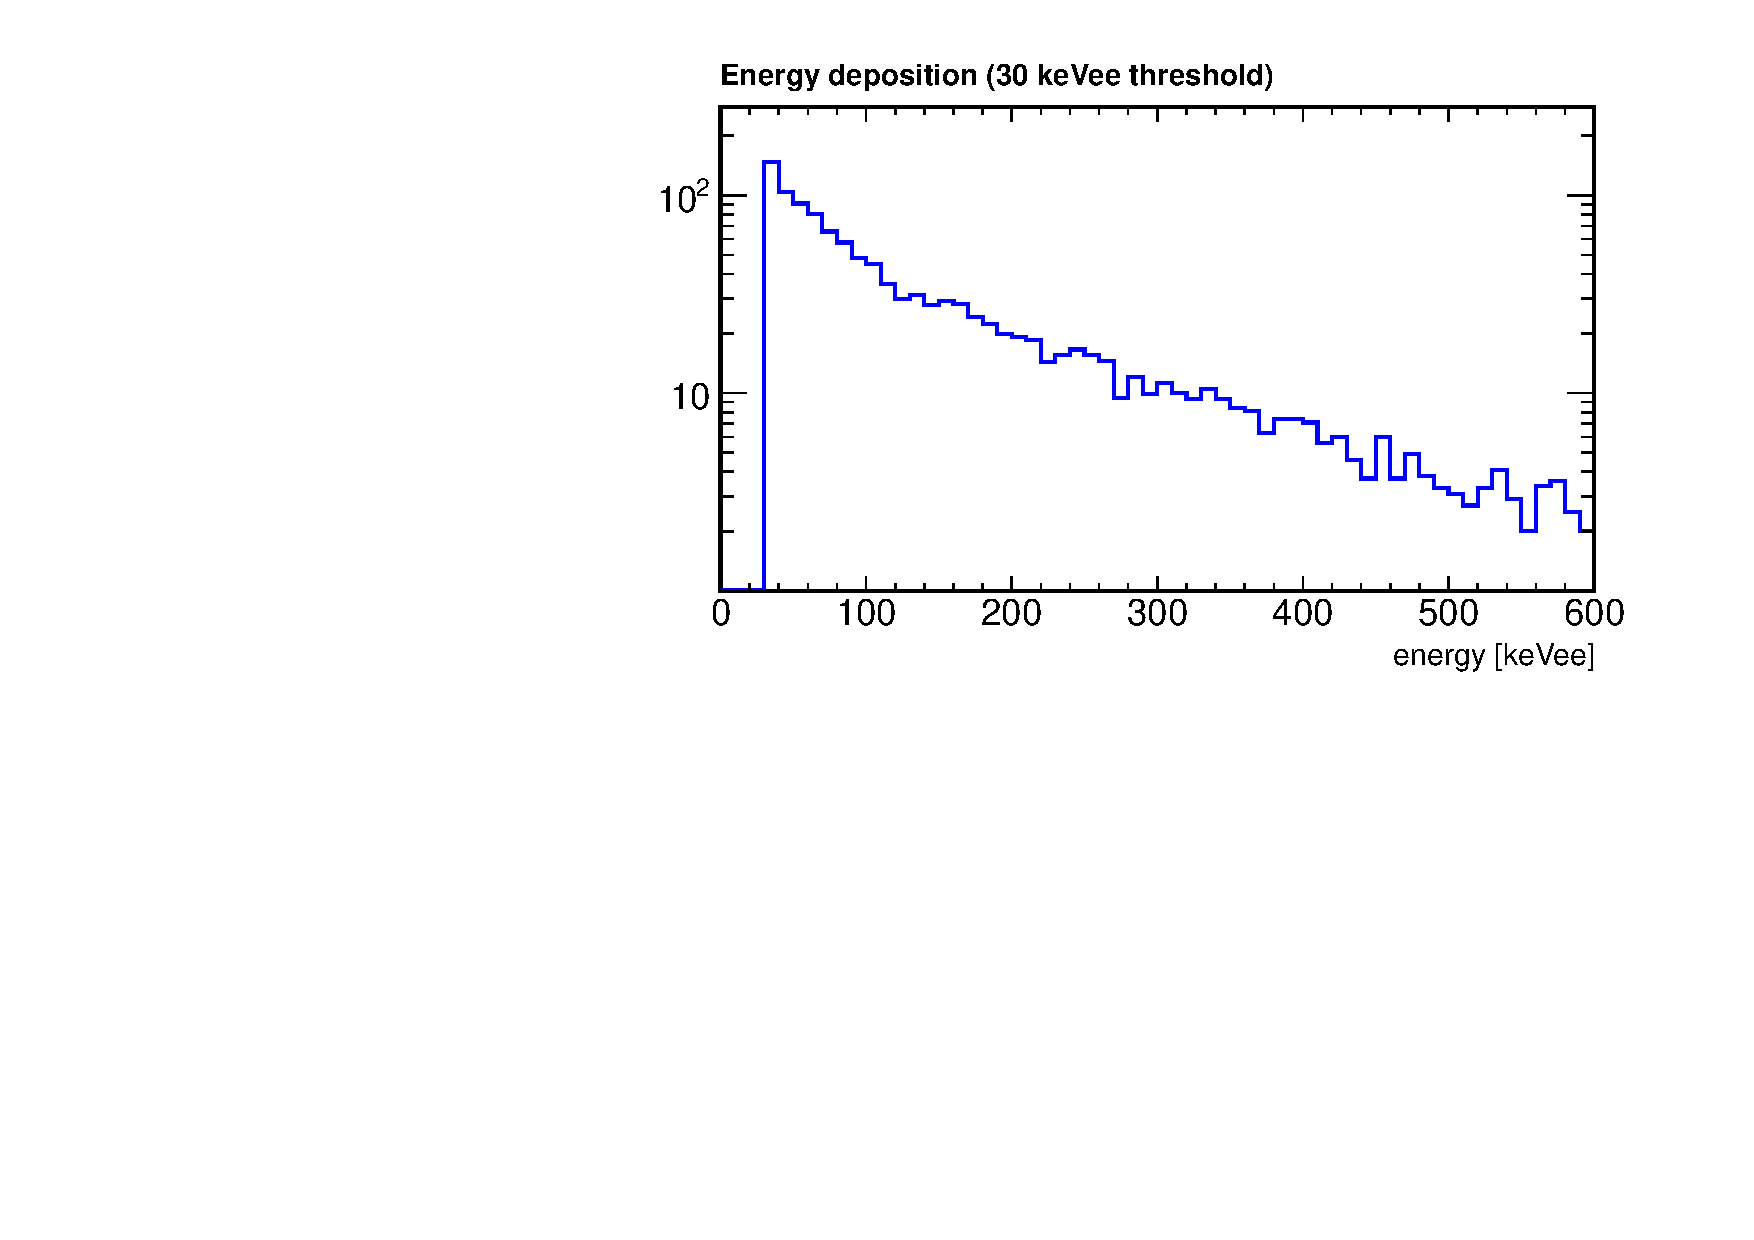
\includegraphics[trim = 0cm 0cm 0cm 1.15cm, clip, width=\textwidth]{pics/edep.pdf}
 		\caption{Timing of Geant4 simulation.}
 	\end{subfigure}
 	\begin{subfigure}[t]{0.49\textwidth}
 		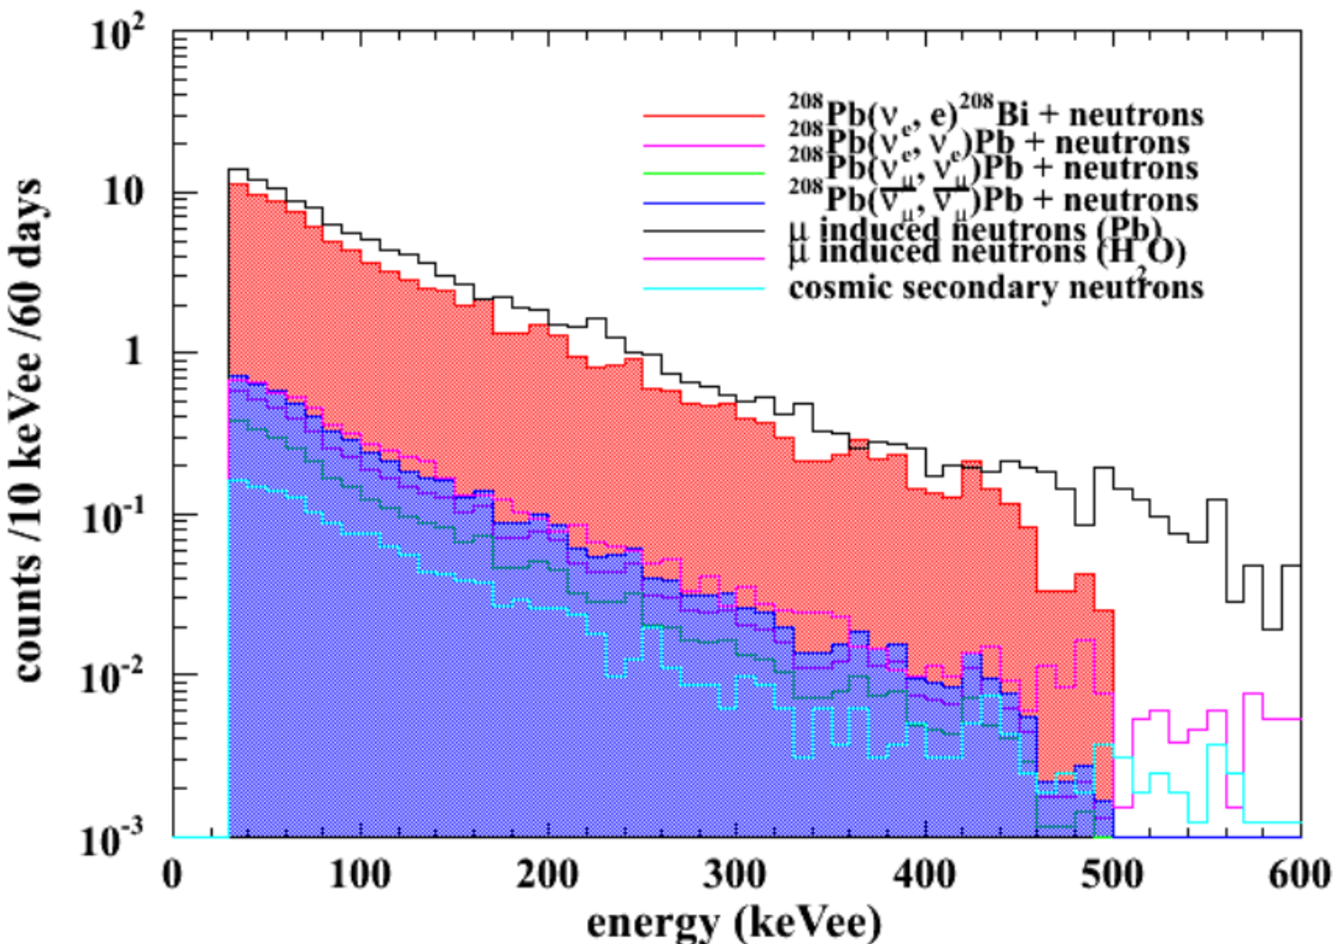
\includegraphics[trim = 0cm 0cm 0cm 1.15cm, clip,width=\textwidth]{pics/edep_MCNP.pdf}
 		\caption{Timing of MCNP simulation.}
 	\end{subfigure}
 	\caption{Threshold \SI{30}{keVee}}
 	\label{fig:edep30}
 \end{figure}
 
\section{Conclusion}


\section*{Acknowledgments}
\begin{itemize}
  \item[] Kate Scholberg and the Duke Neutrino Group.
\end{itemize}

\bibliographystyle{my_utphys}
\bibliography{Final}

\end{document}
